\chapter{Design di dettaglio}

Dopo aver descritto l’architettura del sistema si procede con il design di dettaglio delle sue componenti principali. 
L’approccio progettuale utilizzato combina aspetti Object-oriented, come l’utilizzo dell’interfaccia come astrazione attraverso la quale caratterizzare i componenti, per scatenare comportamenti diversi su entità soggette ad un comune contratto, con elementi di programmazione funzionale pura, quali la tendenza all’impiego di strutture dati immutabili e la riduzione di side effects, favorendo la descrizione lazy della computazione, la separazione fra componente strutturale e comportamentale delle entità ed altri elencati di seguito.


\section{Core}

\section{SimulationEngine e monadi}
Il motore della simulazione \code{SimulationEngine} consiste in una descrizione monadica delle fasi della simulazione, che prevede l’aggiornamento dei parametri del mondo, il rilevamento e risoluzione delle collisioni fra le entità che lo popolano, la visualizzazione a video del suo stato aggiornato e l’attesa dell’intervallo di tempo prima della successiva iterazione. In questo modo il codice non contiene i side-effect invece presenti in un’equivalente versione procedurale, e la parte non funzionalmente pura è confinata, per quel che riguarda il core, all’avvio della applicazione. 
Questo andamento sequenziale e periodico è stato modellato attraverso una composizione di state monad \code{State[World, A]} (per quanto riguarda l’aggiornamento della struttura del mondo) e di IO monad (per le operazioni di I/O come il display a video delle entità e delle statistiche storiche alla chiusura dell’applicazione). Per tale motivo (e a fini di leggibilità) sono stati definiti i seguenti type alias:



\begin{verbatim}
MISSING SNIPPET
\end{verbatim}

La IO monad permette di esprimere una computazione in modo lazy, e in più, la state monad consente di rendere implicito il passaggio di stato aggiornato fra le operazioni sequenziali di manipolazione del mondo, ciascuna delle quali determina una sua nuova versione. Al fine di combinare 2 monadi differenti, che in quanto tali non si possono comporre fra di loro\footnote{Rúnar Bjarnason and Paul Chiusano. Functional Programming in Scala. Exercise 12.11.}, è stato utilizzato il monad transformer \code{StateT: (StateT[SimulationIO, World, A])}.

\begin{verbatim}
MISSING SNIPPET
\end{verbatim}

\section{Queriable type class e ad-hoc polimorphism}
Di supporto alla gestione delle collisioni è definita la typeclass Queriable, che permette ad un type functor di acquisire la capacità di essere interrogabile sulla presenza di un dato elemento al suo interno. La disponibilità in scope di una conversione implicita da qualsiasi funtore di un tipo generico a Queriable gli permette non solo di verificare se un elemento di tale tipo generico è da esso contenuto, ma di abilitare una serie di algoritmi già implementati e riusabili (fra i quali containedAnyOf e containedAllOf). La possibilità di abilitare a posteriori tali conversioni implicite rende questa astrazione (e l’insieme degli algoritmi che la sfruttano) applicabile retroattivamente a tipi già esistenti, oltre che a quelli futuri, offrendo un meccanismo di ereditarietà più flessibile dell’ereditarietà. Per implementare la type class, che in scala non è attualmente disponibile come astrazione di prima classe, e attivare il meccanismo di conversione implicita sono stati sfruttati gli higher-kinded-type assieme ai context-bound.

\section{Model}

\subsection{Struttura entità con mixin}
Per la modellazione degli aspetti strutturali delle entità del \code{World} si è sfruttato il meccanismo dei self-type al fine di rendere modulare l’acquisizione di ogni singola caratteristica genetica della popolazione attraverso l’algoritmo di linearizzazione predisposto da scala. Una volta definiti, con un’ottica molto granulare, un set di proprietà e i self-type corrispondenti, attribuendo a ciascuno di essi un dominio minimale ed una singola proprietà/funzionalità, la definizione della componente strutturale delle entità richieste dai requisiti si riduce ad un’attività di composizione di moduli elementari. Ciò porta ad una struttura composta da più livelli di componenti, alcuni dei quali condivisi da più entità. Questo approccio rende riutilizzabili in futuro le astrazioni già definite permettendo di combinare i diversi tratti genetici con flessibilità.

\begin{figure}[h!]
\centering
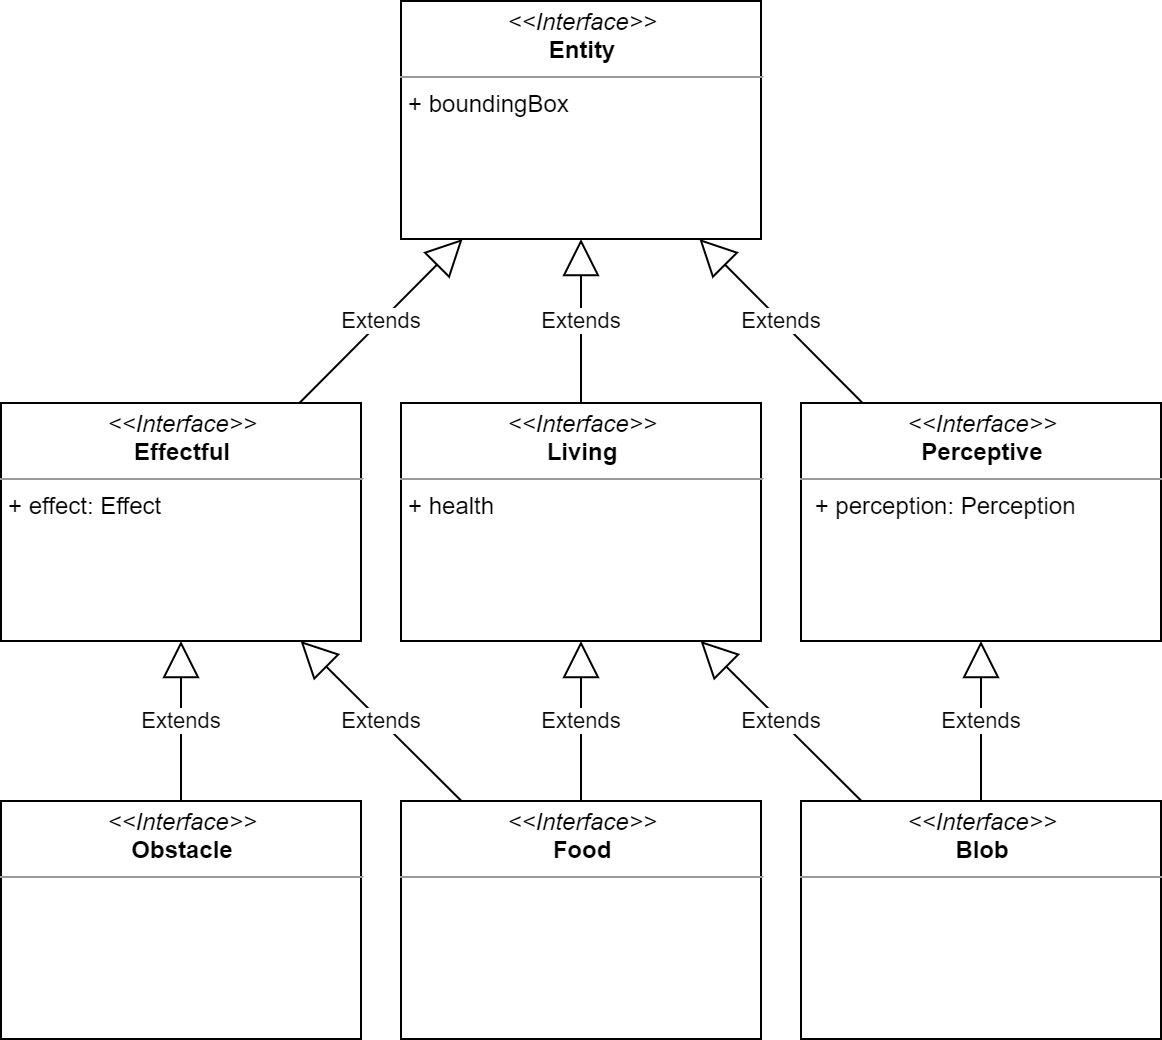
\includegraphics[width=\textwidth, scale=0.44]{img/ModelHierarchy.png}
\caption{Dettaglio UML sulla gerarchia strutturale delle entità della simulazione. Ciascun astrazione identifica una singola funzionalità.}
\label{fig:modelhierarchy3}
\end{figure}

Come proprietà della struttura sono utilizzati diversi parametri higher order (come \code{MovementStrategy}, \code{DegradationEffect} e \code{CollisionEffect}), che fungono da strategie e definiscono il comportamento dell’entità per aspetti specifici (la degradazione della propria vita o il movimento all’interno dell’area di simulazione, ad esempio). Ciò permette di riutilizzare una stessa struttura per modellare una serie di comportamenti diversi, piuttosto che codificare tale diversità di comportamento nel codice, trasferendola dunque a livello di istanza anziché di classificazione (dall’aspetto intensionale a quello estensionale). Invece di esprimere nel codice di una entità la logica di alcuni aspetti specifici, si incapsula dunque tale gestione in un parametro higher order, permettendo ad esempio di riutilizzare anche per entità con diverse logiche di degradazione la struttura rimanente. Al contempo, chiunque vorrà estendere il sistema di simulazione in futuro potrà usufruire di tali strategie per l’implementazione delle sue componenti.

\subsection{Comportamento entità con self type}
L’aspetto comportamentale delle entità, che riguarda cioè le operazioni che agiscono sul loro stato in occasione dell’evento di aggiornamento del mondo e di collisione con altre entità, è gestito mediante 2 trait con self types: \code{Updatable} e \code{Collidable}. Questa modellazione prevede di sfruttare la interfaccia per variare il comportamento sotto la stessa astrazione e fornire estendibilità futura e, al contempo, un approccio funzionale nella gestione dello stato (ogni entità è immutabile e l’aggiornamento coincide con la generazione di una nuova versione con proprietà modificate). Le signature di \code{Updatable} e \code{Collidable} prevedono di restituire un set di \code{SimulableEntity} che rimpiazza l’entità nell’iterazione successiva e permette di esprimerne la rimozione, l’aggiornamento o eventi quali la riproduzione o la clonazione della stessa.

\begin{figure}[h!]
\centering
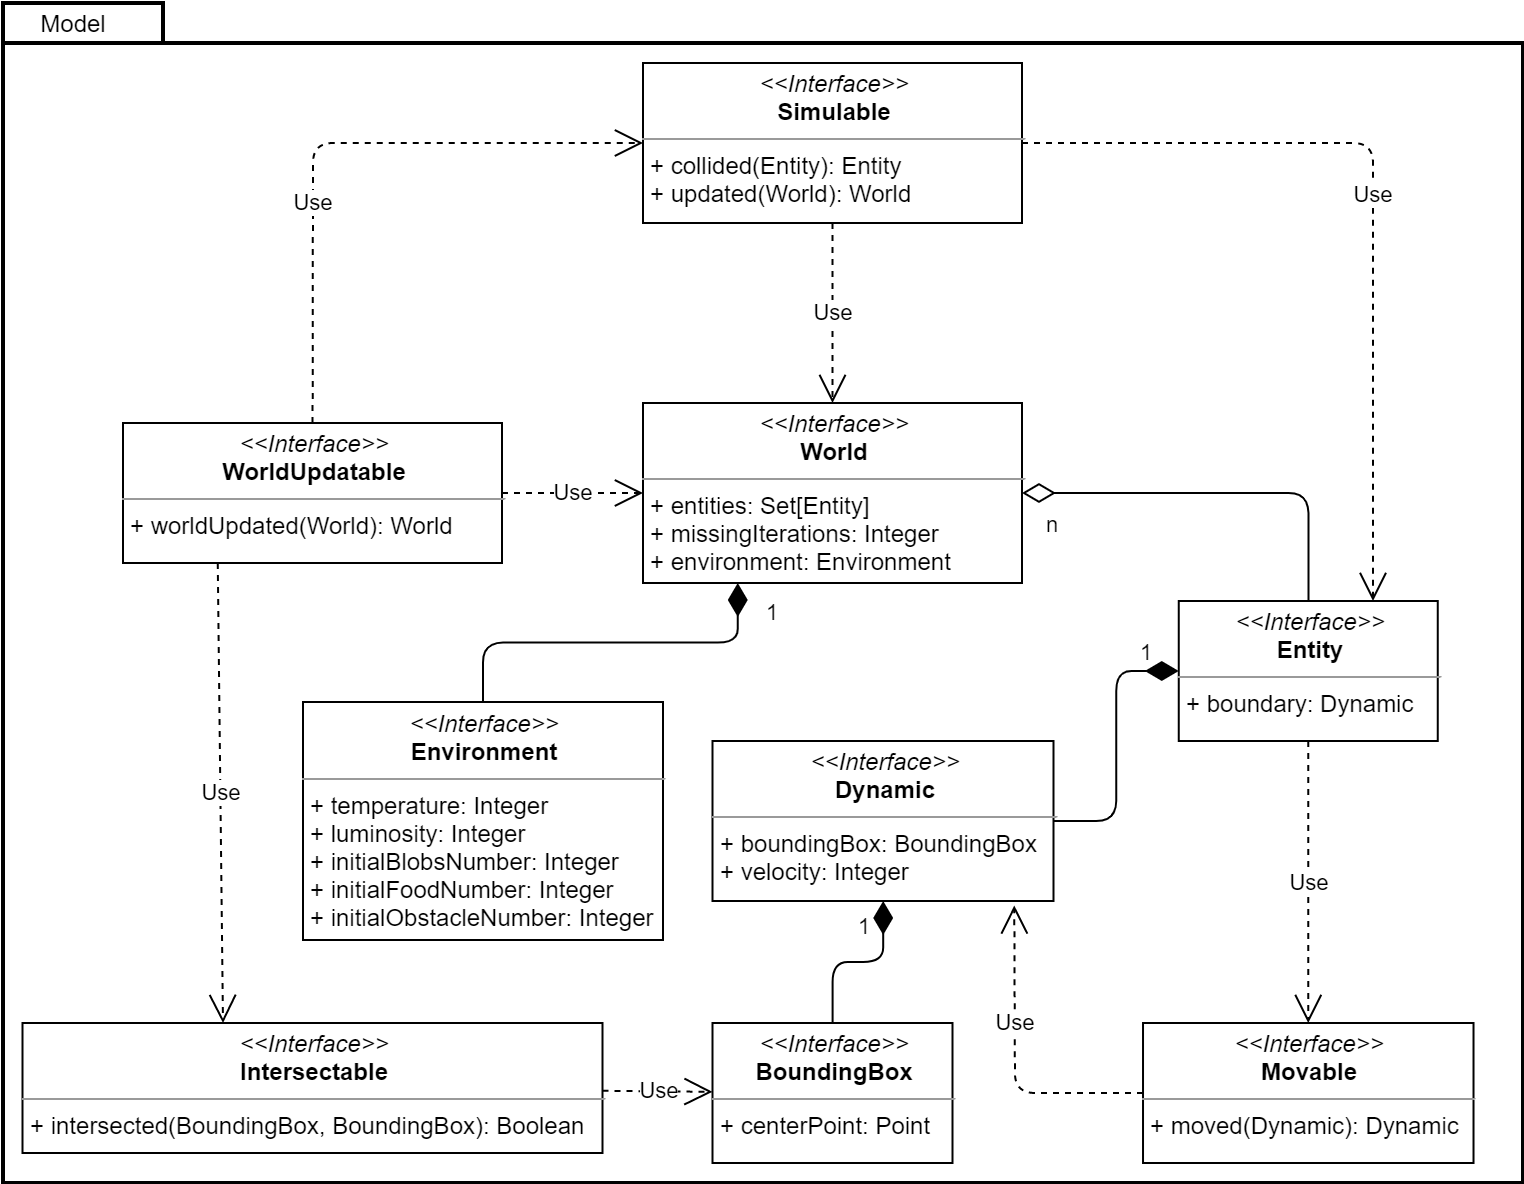
\includegraphics[width=\textwidth, scale=0.14]{img/Model.png}
\caption{Design Model}
\label{fig:model}
\end{figure}

Il requisito che un’entità deve soddisfare per partecipare ad una simulazione si suddivide in 2 componenti, rappresentati dal type alias \code{SimulableEntity}: dal punto di vista strutturale il vincolo di rappresentare una Entity, mentre, dal punto di vista comportamentale, quello di disporre di un’implementazione di tali 2 trait, la cui unione è definita mediante il type alias \code{Simulable}.

\begin{verbatim}
MISSING SNIPPET
\end{verbatim}

A tale scopo, i companion object di \code{Updatable} e \code{Collidable} forniscono delle implementazioni dei rispettivi trait pronte all’uso per comportamenti riusabili e applicabili intercambiabilmente a qualunque Entity. (\code{NeutralUpdatable} e \code{NeutralCollidable} definiscono dei comportamenti che decorano i tipi sottostanti non inducendo nessuna modifica nella entità su cui vengono installati). Per questo motivo, in ottica futura, l’implementazione di Entity è sufficiente a disporre di nuove entità potenzialmente integrabili all’interno della simulazione.

\section{View}

Le operazioni di input e output della view consistono in descrizioni monadiche lazy della costruzione e comportamento dei componenti, così da aderire al paradigma funzionale nonostante la tipica natura object-oriented dei componenti di View. Sono state individuate un'operazione di input e due di output. La prima consiste nella lettura dei parametri di inizializzazione della simulazione contenuti in un oggetto \code{Environment} che verrà usato per la costruzione del \code{World}. La prima operazione di output viene richiamata ad ogni iterazione e fornisce lo stato attuale del \code{World} e delle entità che lo popolano. L'ultima, dato lo storico di tutte le istanze di \code{World} in modo lazy, provvede all'aggregazione delle informazioni contenute per fornire statistiche sulla simulazione.

\section{Pattern di progettazione}
Il team ha cercato di utilizzare il più possibile i pattern di progettazione, al fine di trovare una soluzione di design generale a problemi ricorrenti. Questo approccio si è rivelato efficace nel contenere o ridurre il debito tecnico.
\subsection{Strategy}
È stato ampiamente utilizzato il pattern Strategy all’interno del progetto, in quanto supportato nativamente dal linguaggio scala come passaggio di funzioni higher-order.
\subsection{Self-Type}
I \textit{self types} come accennato nella sezione [4.2.3] sono stati utilizzati per l'implementazione dei seguenti behaviour:
\begin{itemize}
    \item \code{NeutralBehaviour}
    \item \code{BaseBlobBehaviour}
    \item \code{CannibalBlobBehaviour}
    \item \code{TemporaryStatusBlobBehaviour}
    \item \code{BaseFoodBehaviour}
    \item \code{StandardPlantBehaviour}
    \item \code{ReproducingPlantBehaviour}
    \item \code{PoisonousPlantBehaviour}
\end{itemize}
\subsection{Singleton}
Abbiamo ampiamente utilizzato il pattern Singleton nel progetto, in quanto Scala rende particolarmente semplice l’implementazione dello stesso.
\subsection{Factory}
Nel progetto si è fatto uso del pattern Factory per la creazione di oggeti quali ad esempio le \code{BoundingBox} facendo uso del suo companion object.
\subsection{Builder}
Come altri pattern anche il Builder è stato utilizzato nella sua accezione legata a Scala, in quanto ha un supporto nativo per differenti pattern progettuali. Nello specifico per il pattern Builder è stato sfruttato l’utilizzo di immutable case classes con default nei parametri dei costruttori come ad esempio per i \code{Blob} in \code{Entities}.

\section{Organizzazione del codice}
Il sistema è stato organizzato in package ognuno dei quali raggruppa i sorgenti che implementano una specifica feature. La Figura \ref{fig:pakage} mostra la suddivisione effettuata per il progetto e per chiarezza visiva quelli meno importanti sono stati omessi.

\begin{figure}[h!]
\centering
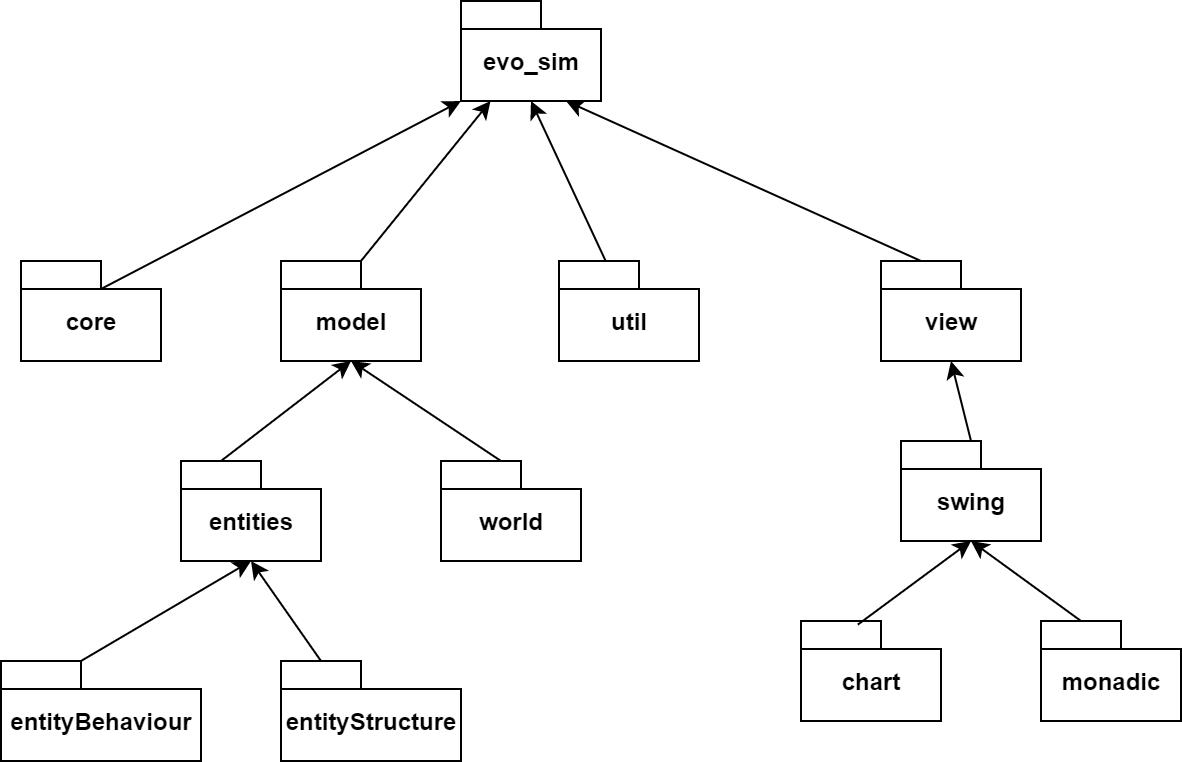
\includegraphics[width=\textwidth, scale=0.44]{img/Packages.png}
\caption{Diagramma strutturale del progetto}
\label{fig:pakage}
\end{figure}
